\chapter{Implementation}
\label{ch:implementation}



This chapter describes the implementation of the concepts explained in chapter \ref{ch:approach}.
Parts of the system were already implemented by other developers before this thesis.

As stated in section \ref{sec:architecture_review} parts of the functionality are still missing and need to be implemented.
This chapter documents the design and implementation of the explained shortcomings.
\\

The following sections of the thesis differ slightly from the proposed time schedule and task list, which was originally planned in the thesis proposal.
In Section \ref{sec:time_schedule} we explain why we had to alter the original thesis schedule based on the findings of the architecture review in section \ref{sec:architecture_review}.


In section \ref{sec:revised_solution_design} we describe how the missing parts of the platform are designed and implemented.
Possible problems or new insights found during this process are explained and dealt with.



\section{Thesis Time Schedule}
\label{sec:time_schedule}
The time schedule of the thesis had to be altered to allow for more time designing and implementing the Basilisk platform.

Before starting this thesis it was hard to quantify how much implementation work was still needed.
After the in-depth architecture review (\ref{sec:architecture_review}) it became clear that the implementation workload was greater than anticipated in the thesis proposal.

Therefore an alteration of the time schedule and work plan for the thesis is needed.
Further we discuss the task priorities.
First priority is the development of the core functionality for the platform.
This means the main services are required to successfully register new versions of observed repositories, perform benchmark jobs and save the measured metrics to a \ts{}.


With a lower priority, functionalities like user management (\ref{sec:review_user_management}) will be dealt with.
The least priority has the Basilisk frontend (\ref{sec:basilisk_frontend}), since it is not necessarily needed to run the platform.
Secondly it introduces more programming languages and frameworks to the project.
Currently time schedule for the thesis can not provide enough time to fully acquire the understanding for this technology stack.
Therefore the frontend will not be further implemented and deployed in the context of this thesis.


%%%%%%%%%% SOLUTION DESIGN
\section{Revised Solution Design}
\label{sec:revised_solution_design}

The Basilisk platform is missing some key functionality to successfully run benchmark jobs.
In this section we describe the designed solutions for the shortcomings listed in section \ref{sec:architecture_review}.



\subsection{Code Refactoring}
\label{sec:impl_code_refactor}
As stated in section \ref{sec:code_refactor}, an in-depth code refactoring was recommended.
Before starting to design and implement new functionality, we performed an in-depth refactoring and restructuring of the code base.
This created a clean code base on which all future implementations can be build on.

Code refactoring is the process of restructuring the source code of an application without changing its functionality\cite{fowlerRefactoringImprovingDesign2019a}.


\subsection{Management of Repositories and Configurations}
\label{sec:management_repo_config_design}
Section \ref{sec:management_repo_config} already explains the problem of storing and managing repositories, the corresponding hooks and the \ts{}-configurations between the \acf{hcs} and the \acf{jms}.

We discussed different possible solutions, of moving functionality or merging the functionality of the two services into one.
\todo[inline,color=green]{Ist so ein Satz okay der den Denkprozess erklärt? oder nur das Ergebnis erklären?}

In the designed solution, the management and storing of the repositories is moved into the \ac{jms}.
This includes the corresponding REST endpoints and internal logic of the \ac{hcs} that are needed for the management.
The different repositories (\gh{} and \dockh{}) will then be added over the REST API of the \ac{jms}.

In section \ref{sec:review_missing_impl} (\acl{hcs}) it is listed, that the \ac{hcs} is missing the REST endpoints for deleting repositories.
Since the repository management is moved to the \ac{jms}, these endpoints also need to be added there.
\\

The \ac{jms} will communicate with the \ac{hcs} over RabbitMQ message queues.
Through these messages the \ac{hcs} will get the needed information about the repositories it should observe.
These include the URL and for \gh{} repositories details like the observed branch and potentially an OAuth token.

The functionality used when a new release is found, does not need to be changed.
When a new release is found, the \ac{hcs} still sends a message containing the relevant information to the \ac{jms}.
\\

Figure \ref{fig:repo_management_restructure} shows the restructured REST APIs and the adjusted messaging between \ac{hcs} and \ac{jms}.

\begin{figure}[tbph]
	\centering
	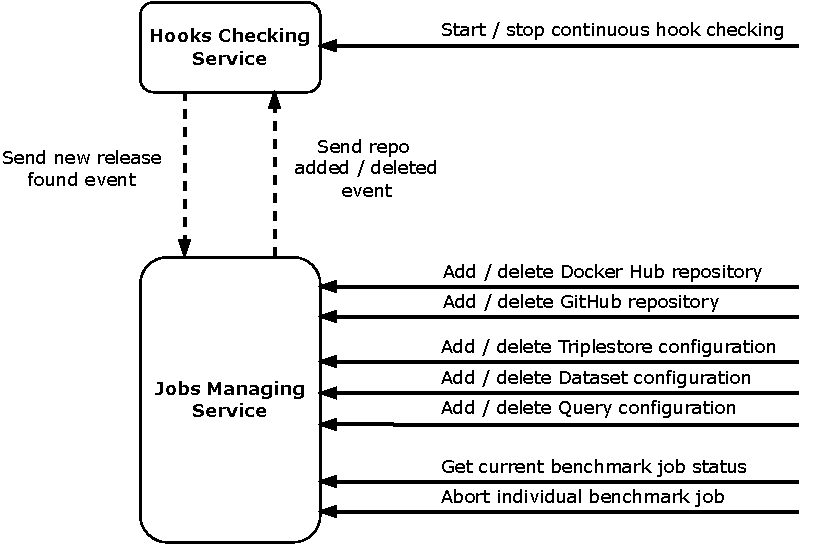
\includegraphics[width=.65\textwidth]{figures/messaging-implementation-hcs-jms.pdf}
	\caption{Overview of the restructured REST APIs and adjusted messaging}
	\label{fig:repo_management_restructure}
\end{figure}



\subsection{Restructure of Data Models in the \acl{jms}}
\label{sec:data_model_restructure_jms}
In section \ref{sec:review_data_model} we reviewed the data model used for storing and managing the different configuration types inside the \ac{jms}.
To mitigate the stated problems with the data model, we designed the database schema shown in figure \ref{fig:design_jms_db_schema}.

\begin{figure}[tbph]
	\centering
	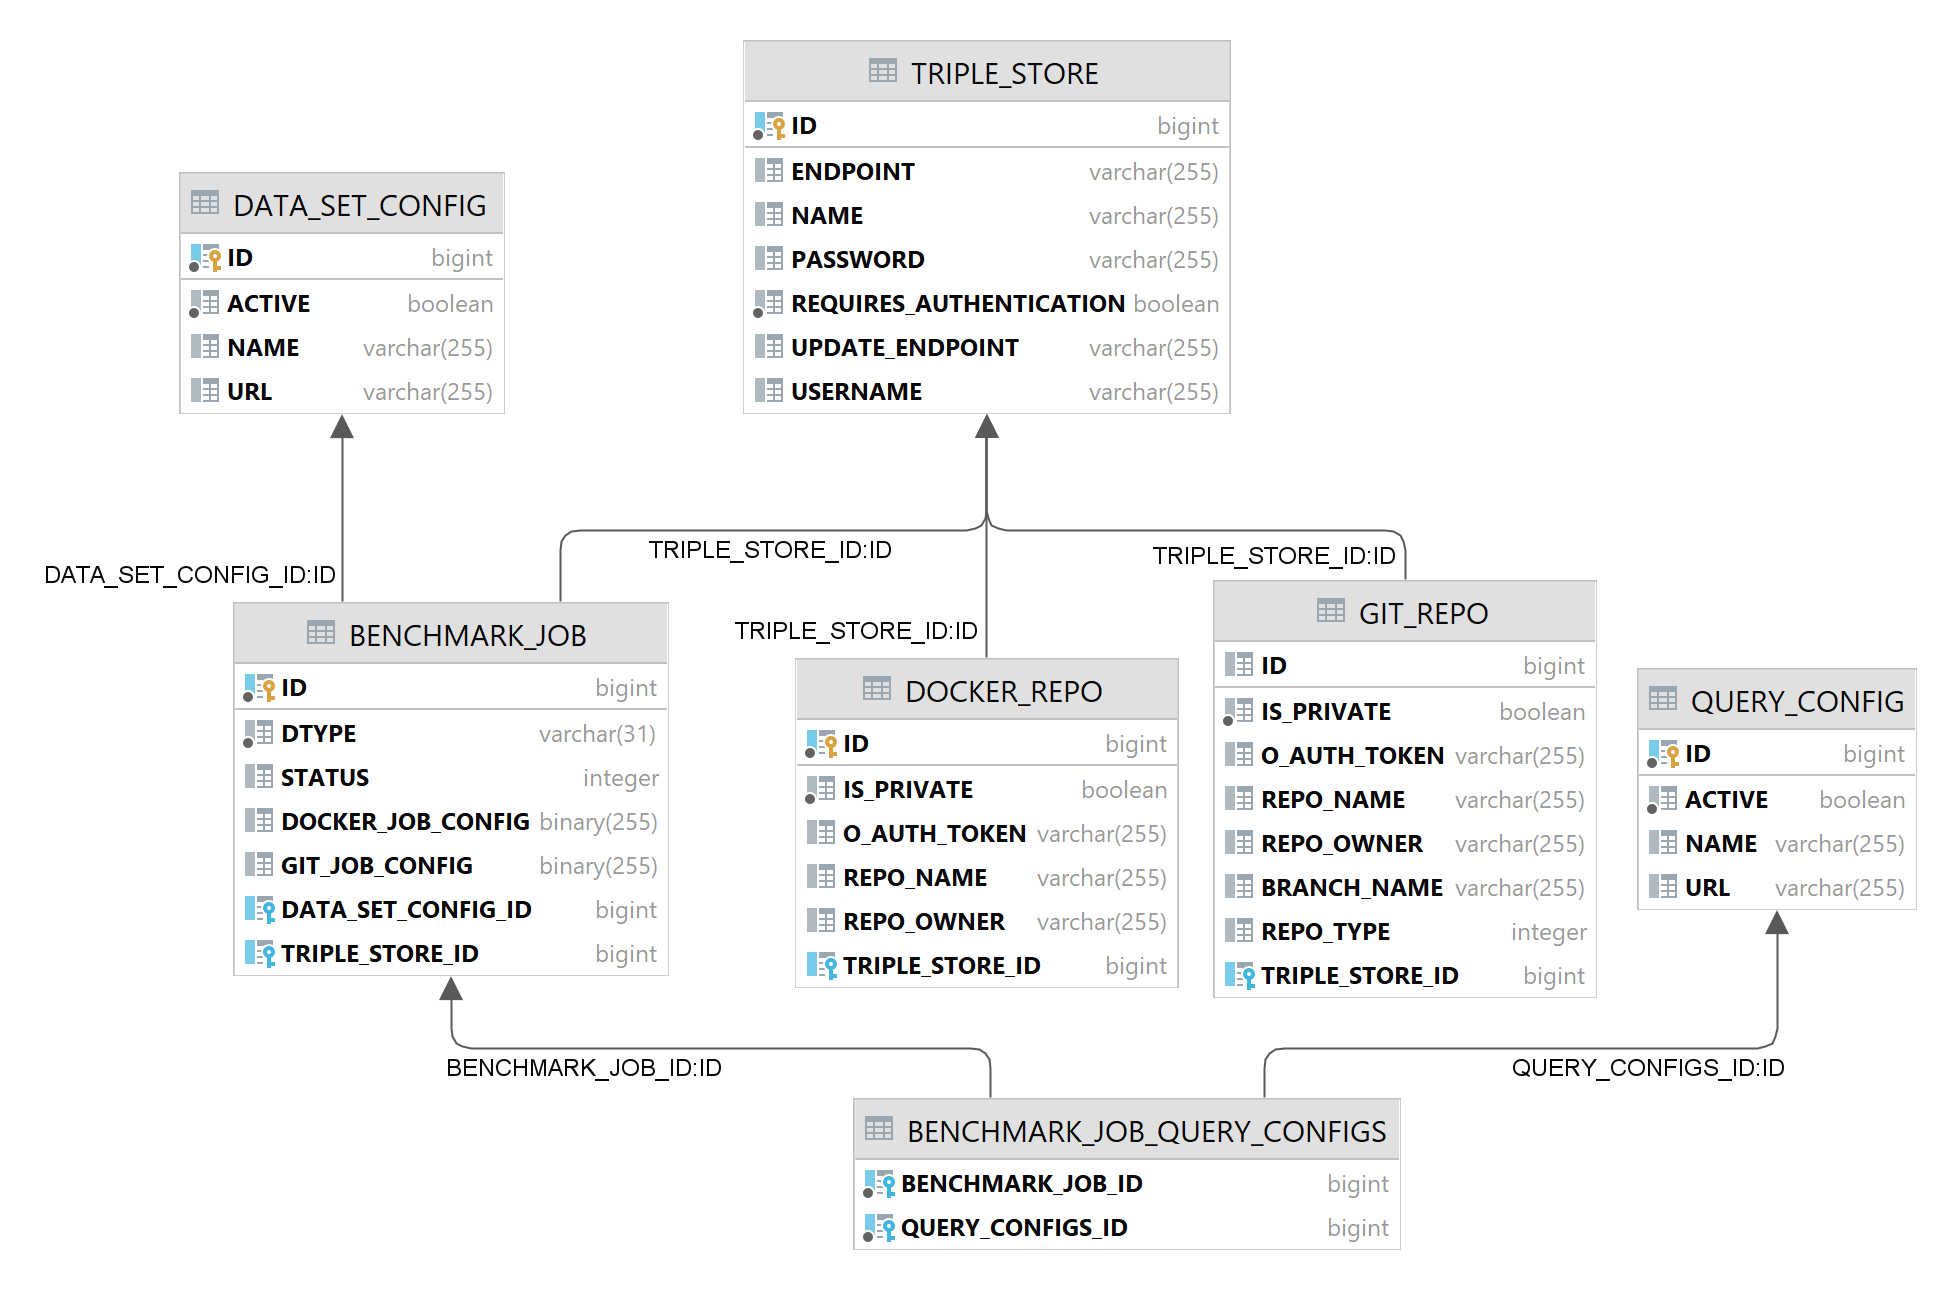
\includegraphics[width=.95\textwidth]{figures/jms_db_schema_design.png}
	\caption{Diagram of the proposed database schema for the \ac{jms}}
	\label{fig:design_jms_db_schema}
\end{figure}

In this design we introduce two different repository types.
One for \gh{} and one for \dockh{}.
This ensures that a repository is always correctly referenced when creating a new benchmark job.

Secondly the relationship between \ac{ts} configurations and repositories is inverted. 
Now each setup repository points to a \ac{ts} configuration.
This means a \ac{ts} configuration can be used for different observed repository setups.

\todo[inline]{changes to benchmark job and dataset/query configs?}


\subsection{Hooks for Pull Requests in \gh{} Repositories}
Currently the Basilisk platform can not check for new pull request published to an observed repository.
This functionality would greatly support the continuous benchmarking during the development process of \tsp{}.

As explained in chapter \ref{ch:approach}, \tsp{} are often developed by teams who collaboratively work on Git repositories.
A standard way of introducing a newly developed feature to a source code repository is a pull request.
Pull requests contain a description of the proposed changes, as well as the name of the development branch which should be pulled into the main branch of the repository.

Often these changes are developed in a forked repository.
A forked repository is basically an independent copy of the main repository.
\gh{} provides functionality to merge the latest changes of the original repo into the forked repo.
To send changes from the forked repo to the original repo, a pull request is needed.

In this forked repo the developer can work independently on his changes and later create the pull request to the original repository.

The difficulty for the Basilisk platform is, that these pull requests can stem from these forked repositories.
Since the repository containing the changes has a different URL to the original repo observed by the Basilisk platform, more information than usual are required to create and run a benchmark job for a pull request.
\\

The solution we designed for this issue is an extended message.
This message gets send in the situation in which the pull requests originates from a different repository.
The message contains the URL, repository and branch name for the \gh{} repository.
Therefore the message handling in the \ac{hcs} and \ac{jms} needs to be adjusted to handle this new message type.

The benchmark jobs and the \acl{tbs} does not need to be changed.
It is not relevant for a benchmark if the repository, from which the docker container is build, is different too the observed repository.


\subsection{Missing Implementations}
\todo[inline,color=green]{Soll ich auch beschreiben, wie ich die fehlenden REST APIs "designed" habe? Oder reicht kurzer Text im Implementation Teil?}
- JMS extend APIs?

- TBS design docker setup flow??





%%%%%%%%%% DEPLOYMENT
\section{Deployment}
\label{sec:deployment}
After the implementation phase, the Basilisk platform is deployed on a virtual server.
The virtual server used is provided by the IRB (Informatik Rechnerbetrieb) of the Computer Science Department at Paderborn University.
Figure \ref{fig:vm_specs} shows the specification of the VM.
The VM was configured to have sufficient resources for small- to medium sized benchmarks.

\begin{figure}[tbph]
	\centering
	\begin{tabular}{ll}
		\toprule
		\textbf{Specifications} &                             \\ \midrule
		CPUs                    & 16 cores                    \\ \midrule
		Memory                  & 128GB                       \\ \midrule
		Storage                 & 2TB                         \\ \midrule
		Operating System        & Debian GNU/Linux 11 (64bit) \\ \bottomrule
	\end{tabular}
	\caption{Specification of the virtual machine on which the platform is deployed.}
	\label{fig:vm_specs}
\end{figure}

The Basilisk platform consists of the 3 main services described in section \ref{sec:main_services}.
For the communication between these services, the platform also needs a RabbitMQ message server.
Also, a \ts{} is required as the \acl{jsts} for storing the benchmark results.
\\

For the platform to be easily manageable we decided to deploy the whole platform in Docker containers.
This has the advantage of using a single Docker Compose file for configuring the services and the network.

The individual services are compiled into jar files and the Docker build copies them into individual Docker images.
The build of the containers for the \ac{hcs} and \ac{jms} is simple and straight forward.
The container for the \ac{tbs} needs two additional configurations for the service to run.
First, the \iguana{} framework is installed inside the container.
Afterwards, the container is configured in the Docker Compose file to has access to the Docker socket of the server.
This is needed for the service to start and manage the Docker images and containers of the \tsp{} that are getting benchmarked.

The RabbitMQ message server is available as an official Docker container on \dockh{}.
For the \ac{jsts} we decided to use the Fuseki\footnote{\url{https://jena.apache.org/documentation/fuseki2/fuseki-main}} \ts{}, which also is available as a Docker container.
\\

In total the Docker Compose configuration consists of 5 containers that can be started and stopped with simple commands.
During a benchmark a sixth container is started which is running the \ts{}.
An overview of the setup is shown in figure \ref{fig:docker-setup}. 

\begin{figure}[tbph]
	\centering
	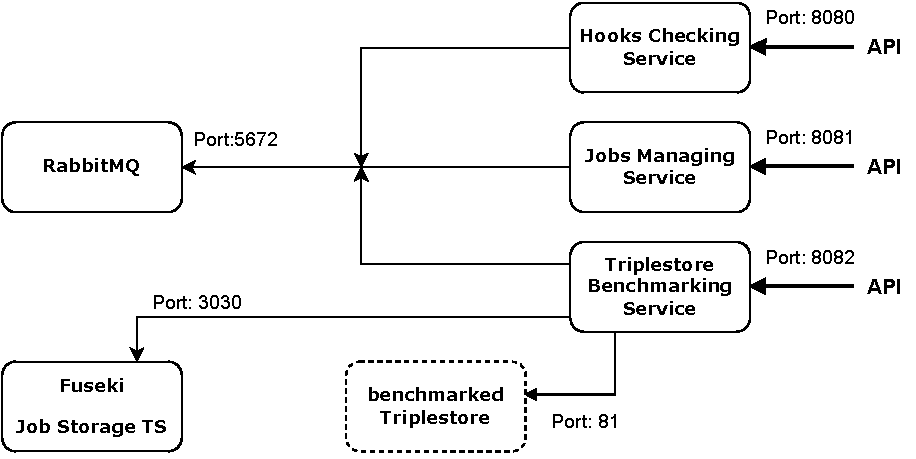
\includegraphics[width=.7\textwidth]{figures/docker-setup.pdf}
	\caption{Overview of the deployed Docker containers and used Ports.}
	\label{fig:docker-setup}
\end{figure}

The three microservices of the Basilisk platform are available through the ports 8080 (\ac{hcs}), 8081 (\ac{jms}), and 8082 (\ac{tbs}) of the host server.
RabbitMQ container is available through port 5672 and the Fuseki \ts{} which is used as the Job Storage for the benchmark results is reachable at port 3030 of the host server.
During a benchmark, the tested \ts{} is started in its own Docker container which also has port 81 published for reaching the SPARQL endpoint.


%%%%%%%%%%%%%%%%
% - Solution design and implementation
% - Deployment of the service
% - Implement benchmarking using IGUANA

% - Design patterns
	